\documentclass[11pt]{article}
\usepackage[T1]{fontenc}
\usepackage{lmodern}
\usepackage[margin=1in]{geometry}
\usepackage{amsmath,amssymb}
\usepackage{booktabs}
\usepackage{graphicx}
\usepackage{microtype}
\usepackage{xcolor}
\usepackage{seqsplit}
\usepackage[hidelinks]{hyperref}
\usepackage[numbers,sort&compress]{natbib}
\hypersetup{
  pdftitle={When Corrections Make Predictions Worse: Preregistered Negative Results for Universal Interatomic Potentials},
  pdfauthor={Alex Welcing, Lupine Science}
}
\newcommand{\code}[1]{\texttt{#1}}
\newcommand{\sha}[1]{\texttt{\seqsplit{#1}}}
\newcommand{\eV}{\,\mathrm{eV}}
\newcommand{\meV}{\,\mathrm{meV}}
\newcommand{\GPa}{\,\mathrm{GPa}}
\emergencystretch=3em

\title{When Corrections Make Predictions Worse:\\Preregistered Negative Results for Universal Interatomic Potentials}
\author{Alex Welcing\\Lupine Science\\\texttt{alex@lupinesci.com}}
\date{August 3, 2026}

\begin{document}
\maketitle

\begin{abstract}
Negative results are useful only when their denominator, selection rule, and provenance remain visible. We report three correction failures from hash-locked materials-simulation records. First, four foundation machine-learning interatomic potentials (uMLIPs) missed a preregistered $40\meV$ migration-barrier gate: float64 mean absolute errors were $135.0$--$242.5\meV$, or $3.4$--$6.1$ times the threshold, over 26--29 completed paths from a 30-chemistry LiTraj/nebDFT2k panel. The signed errors were directionally imbalanced for three models but were not universally one-sided: CHGNet had 25/28 negative errors, MACE-MP medium 21/29, MACE-MP small 17/26, and MACE-MPA-0 medium 13/28. This corrects an earlier summary that called all 26 MACE-MP-small errors negative. Second, 128/128 CatBench candidate--model baseline cells completed, after which a frozen six-train/six-validation/20-test $\Delta$-correction protocol increased holdout MAE for every model-level test (4/4): $0.69\rightarrow2.27$, $2.11\rightarrow5.01$, $3.24\rightarrow5.00$, and $4.27\rightarrow5.91\eV$. Third, on a separate 16-element elastic benchmark, a global leave-one-out principal-component operator increased mean $C_{ij}$ MAE from $14.55$ to $63.40\GPa$. These results do not establish a universal impossibility theorem for correction. They establish a narrower operational rule: a correction must earn its scope out of sample, and preregistration plus hash-locked failures prevents selection from turning degradation into an apparent success.
\end{abstract}

\section{Introduction}

Foundation uMLIPs make atomistic screening fast enough to apply across broad chemical spaces, but their broad training distributions do not guarantee accuracy in transition states, interfaces, or other high-energy environments. CHGNet and MACE illustrate the foundation-model strategy: a single learned potential is reused across many materials and tasks rather than retrained for each system \citep{deng2023chgnet,batatia2024mace}. Independent work has documented systematic softening away from equilibrium \citep{deng2025softening} and has specifically evaluated foundation models on migration barriers \citep{bheemaguli2026barriers}.

Correction is an attractive response. A small calibration set can be used to shift, rescale, or otherwise repair a model's output. But the same flexibility creates a selection hazard: fit and evaluate on overlapping cases, try enough forms, and a correction can appear beneficial even when it does not transfer. A useful negative result therefore needs at least four things: a frozen gate, explicit train/validation/test separation, failures recorded without imputation, and immutable source identities.

This paper reports three such failures. The first two were preregistered Round-4 campaigns: a solid-state ion migration-barrier test (Z1) and an adsorption-energy $\Delta$-correction test (Z3). The third is a separately locked global-operator result on cubic-metal elasticity. The campaigns differ in observable, chemistry, model, and correction form. We do not pool their numerical errors or claim that one scalar mechanism explains all three. We use them together to ask a methodological question: when does correction become degradation, and what evidence is needed to say so honestly?

\section{Locked evidence and methods}

\subsection{Z1: migration barriers}

The Z1 campaign was frozen on July 18, 2026 under manifest content hash
\sha{0a85044ca84d10e021a0a282987976a3a9e79a611a618470e1638e9105171e40}.
Its acceptance test was migration-barrier MAE $\leq40\meV$ across at least 30 chemistry-held-out paths. The candidate panel is one deterministic path from each of the first 30 lexically ordered chemical systems in the official LiTraj nebDFT2k test split \citep{dembitskiy2025litraj}. The panel file is locked at
\sha{192fe54a5579cc421f6644d5d76fb442c6dfb985f014dc4741549e29052efb68}.
References are published PBE DFT climbing-image NEB calculations, not experiment. Both reference and prediction barriers use
\begin{equation}
E_{\mathrm b}=\max_i E_i-\min_i E_i.
\end{equation}
The execution used FIRE, climbing images, improved tangents, a $5\eV\,\text{\AA}^{-2}$ spring constant, $0.1\eV\,\text{\AA}^{-1}$ force tolerance, and at most 100 steps. Failures were recorded without imputation. Four available models were tested: CHGNet 0.4.2 and MACE-MP small, MACE-MP medium, and MACE-MPA-0 medium under mace-torch 0.3.16.

An initial float32 execution was retained as executed evidence. Because float32 geometry optimization conflicted with vendor guidance, the barrier calculation was rerun end to end in float64 with checkpoint dtype binding. The float32 and float64 aggregate measurement files are independently hash locked. We treat float64 as the primary chain and use the first chain only as a precision-sensitivity record.

Signed error is prediction minus reference; a negative value denotes barrier underprediction. We report the count of negative errors among completed paths and do not relabel failed paths. Importantly, the locked rows do \emph{not} support the sentence ``all 26 completed paths are negative.'' The MACE-MP-small chain contains 17 negative and 9 positive signed errors in both precisions. Throughout this paper, ``not all 26'' is a claim guard, not a stylistic caveat.

\subsection{Z3: adsorption-energy \texorpdfstring{$\Delta$}{delta} correction}

The Z3 campaign was frozen under manifest content hash
\sha{49f5f20e41450697b63b9ff079fe25b5490ba684956c5d68bb37a5d2cd02c494}.
The acceptance test was corrected adsorption-energy MAE $\leq0.1\eV$. Its 32-row panel was drawn from the CatBench BM dataset \citep{catbench2025dataset}, whose structures and energies originate in the GAME-Net study \citep{pablogarcia2023gamenet}. The locked panel digest is
\sha{b434de005e5da46e33e3275ffc8bec2d251b8a52438c1cfe7d6f4f3d8dbb41f4}.
References are VASP 5.4.4 PBE+D2 electronic adsorption energies, not experiment; no vibrational, entropic, or finite-temperature correction is included.

A deterministic family-stratified split assigned 6 candidates to fit, 6 to validation-only form selection, and 20 to confirmatory testing. Four predeclared forms were available per model: a global constant, a family constant, a family size-linear form, and a global size-linear form. Fitting read only the training split, selection read only validation, and final scoring read only the confirmatory split. The raw campaign executed 4 models $\times$ 32 candidates = 128 candidate--model cells; 128/128 completed with no failed cell. The phrase ``128/128'' therefore describes baseline execution completeness. The correction comparison has four independent model-level holdout outcomes, not 128 corrected-versus-raw tests.

The correction report is locked at
\sha{95c4fd245fa3e14ca80ff85fff235ce8f58f43dffce996fbf9bd3254adbf838f}.
The primary comparison is each validation-selected form's MAE on its untouched 20-row holdout against that model's raw holdout MAE.

\subsection{Global elastic operator}

The third record is intentionally kept separate from Z1 and Z3. It is a 16-element cubic-metal elastic benchmark using TensorNet/PBE predictions and $T_{\mathrm{PBE},0\,\mathrm K}$ targets. For each held-out element, a global leave-one-out principal-component bias was fitted on the other 15 elements and applied to the held-out elastic tensor. The source results file is locked at
\sha{3a3febabb0cc457685e736f9d35f779d9dd934a6461bae8a28dc5851eb454157}
and vendored here as a minimal provenance record in \code{global-operator.lock.json}. This record tests one operator on one benchmark. It does not expand the Z1 or Z3 denominators.

\section{Results}

\begin{figure*}[t]
  \centering
  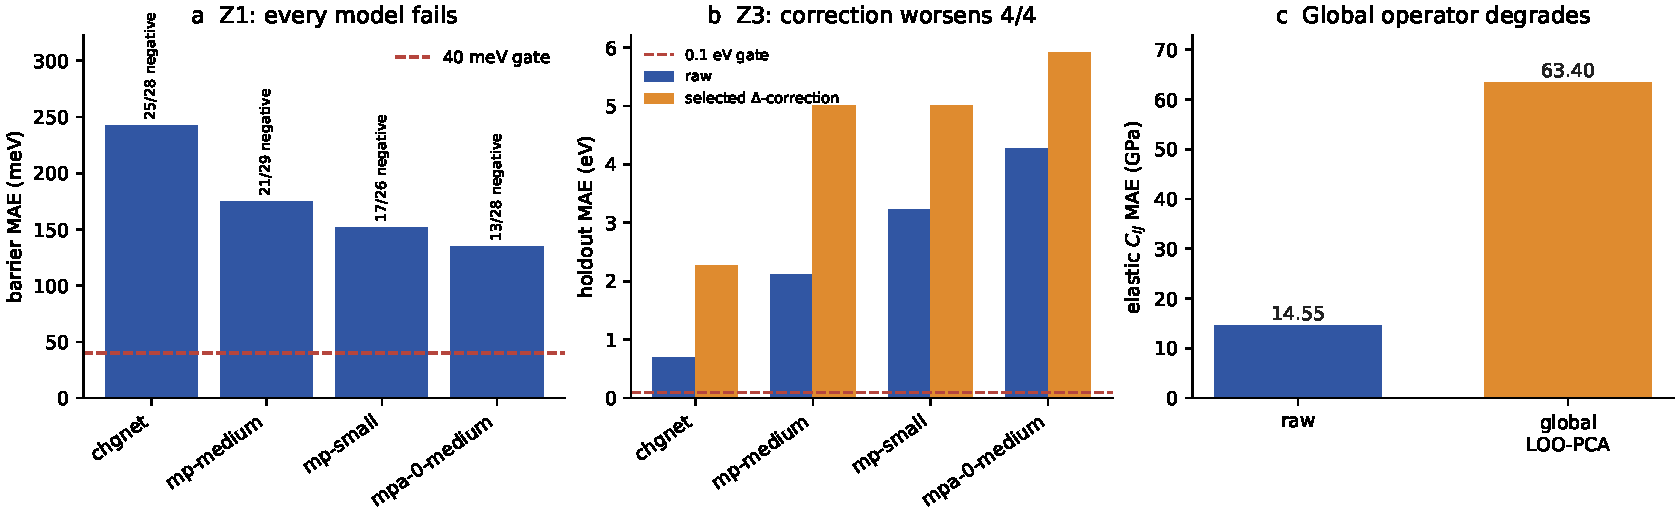
\includegraphics[width=\textwidth]{figures/negative-results-panels.pdf}
  \caption{Three locked negative results. (a) Float64 Z1 barrier MAEs all exceed the preregistered $40\meV$ gate; annotations give negative signed errors among completed paths and show that the directional imbalance is not universal. (b) In Z3, every validation-selected correction increases model-level holdout MAE; 128/128 refers to completed raw candidate--model cells. (c) The separate global LOO-PCA elastic operator increases mean $C_{ij}$ MAE. The plotted values are generated directly from locked inputs by \code{build\_artifacts.py}.}
  \label{fig:results}
\end{figure*}

\subsection{All four Z1 models miss the barrier gate, but the sign claim is bounded}

Table~\ref{tab:z1} reports the float64 chain. Every model fails the $40\meV$ gate, with MAE ranging from $135.0$ to $242.5\meV$---$3.4$--$6.1$ times the threshold. Between one and four paths per model did not converge under the frozen protocol; none was imputed.

\begin{table}[htbp]
\centering
\caption{Z1 float64 results. Signed-error counts are over completed paths only.}
\label{tab:z1}
\begin{tabular}{lrrrr}
\toprule
Model & MAE (meV) & Complete & Negative & Positive \\
\midrule
MACE-MPA-0 medium & 135.0 & 28/30 & 13 & 15 \\
MACE-MP small     & 151.9 & 26/30 & 17 & 9 \\
MACE-MP medium    & 174.7 & 29/30 & 21 & 8 \\
CHGNet            & 242.5 & 28/30 & 25 & 3 \\
\bottomrule
\end{tabular}
\end{table}

The failure is directional for CHGNet and for both MACE-MP variants, but not for MACE-MPA-0 medium. CHGNet's 25/28 negative errors are a strong descriptive imbalance in this panel; MACE-MPA-0 medium's 13/28 are not. The MACE-MP-small mean signed error is $-23.7\meV$ while its MAE is $151.9\meV$, demonstrating that cancellation can hide a large absolute-error burden. The float32 chain yields the same aggregate verdicts to within $0.1\meV$ but does not restore an all-negative MACE-MP-small distribution.

The corrected interpretation is therefore precise: all four models miss the preregistered accuracy threshold, and three show more underpredictions than overpredictions among completed paths. It is not correct to call all completed paths underpredictions, nor to call the $3.4$--$6.1$ quantity an underprediction factor; it is an MAE-to-threshold ratio.

\subsection{Every selected Z3 correction is worse out of sample}

Table~\ref{tab:z3} gives the untouched confirmatory results. Validation selection chose different forms for different models, but every selected form increased holdout MAE. The smallest raw error, CHGNet at $0.69\eV$, became $2.27\eV$. The other models increased from $2.11$--$4.27\eV$ raw to $5.00$--$5.91\eV$ corrected. All corrected results remain far above the $0.1\eV$ gate.

\begin{table}[htbp]
\centering
\caption{Z3 validation-selected corrections on the 20-row confirmatory holdout.}
\label{tab:z3}
\begin{tabular}{llllr}
\toprule
Model & Selected form & Raw (eV) & Corrected (eV) & Change \\
\midrule
CHGNet & family size-linear & 0.69 & 2.27 & worse \\
MACE-MP medium & global constant & 2.11 & 5.01 & worse \\
MACE-MP small & global constant & 3.24 & 5.00 & worse \\
MACE-MPA-0 medium & family constant & 4.27 & 5.91 & worse \\
\bottomrule
\end{tabular}
\end{table}

The failure mode is visible in the signed rows. A constant shift can overshoot candidates whose raw error is small or opposite in sign. A family size-linear form can extrapolate from a tiny within-family fit budget into much larger corrections on the holdout. Because the form was selected on validation and evaluated only once on the held-out 20, this is not a report of failed training fit. It is a report of failed transfer.

\subsection{A global elastic correction degrades every element}

The global LOO-PCA operator increased mean elastic-tensor MAE from $14.5466$ to $63.3952\GPa$, reported as $14.55\rightarrow63.40\GPa$. Its 95\% bootstrap intervals were $[10.08,19.72]\GPa$ raw and $[57.07,69.18]\GPa$ corrected. In the locked benchmark report the corrected per-element MAE exceeds raw MAE for all 16 elements. Leave-one-out fitting prevents direct target leakage, but it cannot make a single global error direction transferable when element-level error directions differ.

\section{Discussion}

\subsection{What the three failures establish}

The shared result is methodological rather than numerical. First, a frozen gate can turn an expensive run into useful evidence even when no model passes. Second, train/validation/test separation is necessary but not sufficient: Z3 obeyed the split and still failed because a six-point fitting budget could not identify a correction that transferred across family and size. Third, leave-one-out fitting is necessary but not sufficient: the elastic operator avoided in-sample fitting and still imposed the wrong global direction.

These results motivate a correction license with three explicit coordinates: observable, material class, and calibration support. A correction validated for one coordinate tuple should not silently transfer to another. The appropriate default outside a validated tuple is abstention or raw reporting, not correction by analogy.

The Z1 sign counts also show why negative results need claim-level locks. A large MAE and a negative mean signed error do not imply that every path is underpredicted. The stale all-26 sentence would have converted an imbalanced distribution into a universal statement. Recomputing the counts from the immutable per-path records exposes the error without changing the campaign outcome.

\subsection{What the failures do not establish}

We do not claim that uMLIPs always underpredict barriers. MACE-MPA-0 medium has more positive than negative Z1 errors on this panel. We do not claim that $\Delta$ learning is generally ineffective; we refute the frozen six-train/six-validation protocol on this CatBench-derived panel. We do not claim that every global operator fails; we report one LOO-PCA elastic operator on 16 cubic elements. We do not merge DFT reference errors with experimental errors, and we do not interpret the CatBench electronic convergence proxy as a statistical uncertainty interval.

The studies also have different reference bases. Z1 uses published PBE CI-NEB barriers. Z3 uses PBE+D2 adsorption energies. The elastic benchmark uses $T_{\mathrm{PBE},0\,\mathrm K}$ targets. Cross-study language is therefore restricted to the observed fact that correction and broad transfer can fail; no common error magnitude is inferred.

\section{Reproducibility and claim lock}

The arXiv source bundle contains the manuscript, bibliography, generated figure, machine-readable figure data, a generated-artifact manifest, and the build/verification script. From the repository root, run:
\begin{quote}
\code{python paper/negative-results-preprint/build\_artifacts.py --check}
\end{quote}
The script fails closed if any of ten source digests changes, including the raw Z3 candidate--model registry and the global-operator lock. It derives Z3 completeness and model-level worsening counts from the locked records, derives the required elastic values from the operator lock, and refuses to build if those values contradict the manuscript. It also refuses to build if MACE-MP small is no longer 17 negative / 9 positive or if any Z3 selected correction ceases to be worse than its baseline.

\begin{table}[htbp]
\centering
\caption{Primary claim locks. Content hashes are the manifests' canonical hashes; file hashes are verified by the build script.}
\begin{tabular}{p{0.25\textwidth}p{0.67\textwidth}}
\toprule
Object & Lock \\
\midrule
Z1 panel & \sha{192fe54a5579cc421f6644d5d76fb442c6dfb985f014dc4741549e29052efb68} \\
Z1 campaign content & \sha{0a85044ca84d10e021a0a282987976a3a9e79a611a618470e1638e9105171e40} \\
Z1 float64 measurements & \sha{550fc6b12c8b34837b552e5e7aa282c35b21893e58d901670c06623c48e82c55} \\
Z3 panel & \sha{b434de005e5da46e33e3275ffc8bec2d251b8a52438c1cfe7d6f4f3d8dbb41f4} \\
Z3 campaign content & \sha{49f5f20e41450697b63b9ff079fe25b5490ba684956c5d68bb37a5d2cd02c494} \\
Z3 correction report & \sha{95c4fd245fa3e14ca80ff85fff235ce8f58f43dffce996fbf9bd3254adbf838f} \\
Elastic source result & \sha{3a3febabb0cc457685e736f9d35f779d9dd934a6461bae8a28dc5851eb454157} \\
\bottomrule
\end{tabular}
\end{table}

\section*{Data and code availability}

All Z1 and Z3 manifests, locked panels, measurement rows, correction code, tests, and local artifact mirrors are included in the Lupine Rhizo repository. The global elastic summary is bound to its source repository commit and source-file digest in \code{global-operator.lock.json}. Cloud artifact URIs and local hash mirrors are enumerated in the Z1 and Z3 artifact manifests. Failed Z1 paths remain explicit and are never imputed.

\section*{Conflicts of interest}

The author declares no competing interests.

\bibliographystyle{unsrtnat}
\bibliography{references}

\end{document}
